
% -*- fill-column: 80; -*-
\documentclass[sigconf,anonymous,review,screen]{acmart}
\usepackage{mathpartir}
\usepackage{tikz-cd}
\usepackage{lipsum}
\usepackage{enumitem}
\usepackage{wrapfig}
\usepackage{fancyvrb}
\usepackage{hyperref}
\usepackage{cleveref}
\usepackage{stmaryrd}
\usepackage{tikz}
\usetikzlibrary{automata, positioning, arrows, fit}

\usepackage{pdfpages}

\newcommand{\sem}[1]{\llbracket{#1}\rrbracket}
\newcommand{\cat}[1]{\mathbf{#1}}
\newcommand{\lto}{\multimap}
\newcommand{\tol}{\mathrel{\rotatebox[origin=c]{180}{$\lto$}}}
\newcommand{\String}{\Sigma^{*}}
\newcommand{\Set}{\mathbf{Set}}
\newcommand{\Gr}{\mathbf{Gr}}
\newcommand{\Type}{\mathbf{Type}}
\newcommand{\Prop}{\mathbf{Prop}}
\newcommand{\Bool}{\mathbf{Bool}}
\newcommand{\nat}{\mathbb{N}}

\newcommand{\gluedNL}{{\mathcal G}_S}
\newcommand{\gluedNLUniv}{{\mathcal G}_{S,i}}
\newcommand{\gluedL}{{\mathcal G}_L}

\newcommand{\simulsubst}[2]{#1\{#2\}}
\newcommand{\subst}[3]{\simulsubst {#1} {#2/#3}}
\newcommand{\letin}[3]{\mathsf{let}\, #1 = #2 \, \mathsf{in}\, #3}
\newcommand{\lamb}[2]{\lambda #1.\, #2}
\newcommand{\lamblto}[2]{\lambda^{{\lto}} #1.\, #2}
\newcommand{\lambtol}[2]{\lambda^{{\tol}} #1.\, #2}
\newcommand{\dlamb}[2]{\overline{\lambda} #1.\, #2}
\newcommand{\app}[2]{#1 \, #2}
\newcommand{\applto}[2]{#1 \mathop{{}^{\lto}} #2}
\newcommand{\apptol}[2]{#1 \mathop{{}^{\tol}} #2}
\newcommand{\PiTy}[3]{\Pi #1 : #2.\, #3}
\newcommand{\SigTy}[3]{\Sigma #1 : #2.\, #3}
\newcommand{\LinPiTy}[3]{\widebar\Pi #1 : #2.\, #3}
\newcommand{\LinSigTy}[3]{\widebar\Sigma #1 : #2.\, #3}
\newcommand{\amp}{\mathrel{\&}}
\newcommand{\GrTy}{\mathsf{Gr}}

\newcommand{\ctxwff}[1]{#1 \,\, \mathsf{ok}}
\newcommand{\ctxwffjdg}[2]{#1 \vdash #2 \,\, \mathsf{type}}
\newcommand{\linctxwff}[2]{#1 \vdash #2 \,\, \mathsf{ok}}
\newcommand{\linctxwffjdg}[2]{#1 \vdash #2 \,\, \mathsf{linear}}

\newif\ifdraft
\drafttrue
\newcommand{\steven}[1]{\ifdraft{\color{orange}[{\bf Steven says}: #1]}\fi}
\renewcommand{\max}[1]{\ifdraft{\color{blue}[{\bf Max says}: #1]}\fi}
\newcommand{\pedro}[1]{\ifdraft{\color{red}[{\bf Pedro says}: #1]}\fi}
\newcommand{\pipe}{\,|\,}

\begin{document}

\pagestyle{plain}

\pagebreak

\title{Formal Grammars as Types in Non-commutative Linear-Non-Linear Type Theory}

\author{Steven Schaefer}
\affiliation{\department{Electrical Engineering and Computer Science}
  \institution{University of Michigan}
  \country{USA}
}
\email{stschaef@umich.edu}

\author{Max S. New}
\affiliation{
  \department{Electrical Engineering and Computer Science}
  \institution{University of Michigan}
  \country{USA}
}
\email{maxsnew@umich.edu}

\author{Pedro H. Azevedo de Amorim}
\affiliation{
  \department{Department of Computer Science}
  \institution{University of Oxford}
  \country{UK}
}
\email{pedro.azevedo.de.amorim@cs.ox.ac.uk}

\makeatletter
\let\@authorsaddresses\@empty
\makeatother

\begin{abstract}
  In this paper, we propose a new syntactic formalism for formal grammars: a
  dependent linear/non-linear type theory in which the tensor product is
  non-commutative. The linear types in this calculus may be interpreted as
  grammars, and linear terms as parse transformers. This provides a logical
  characterization of grammar classes based on a substructural logic rather than
  ordinary first-order logic.

  Internally to our calculus, we carry out many classical constructions from
  the theory of formal grammars. Inspired by the common
  structure underlying various ideas in formal language
  theory, our type theory makes these relationships explicit
  and provides a unifying syntax to reason about formal
  grammars.

  We give this type theory a semantics in the category of grammars and prove a
  canonicity theorem showing that every term in a context corresponding to a
  fixed string is equal to a term in a canonical form encoding a parse tree of
  that string. Finally, we discuss the application to the design and
  implementation of correct-by-contruction parsers.
\end{abstract}

\maketitle

\section{A Syntax-Independent Notion of Syntax}
\label{sec:intro}
The theory of formal languages and parsing is one of the oldest and
most thoroughly developed areas of theoretical computer science. A
prominent topic in the 1950, 60s, and 70s led to a series of remarkable
developments: Chomsky's hierarchy of grammar formalisms \cite{chomThreeModels1956}, practical
algorithms for parsing of regular and context-free grammars and
variants \cite{KNUTH1965607,Earley1970}, as well as implementations of practical tools for the
generation of efficient parsers \cite{Johnsonyacc}.

The notion of formal language is central to the theory of parsing. A
\emph{formal language} $L$ over an alphabet $\Sigma$ is classically defined as a
\emph{subset} of strings $L \subseteq \String$. This definition is
especially useful as it gives a semantics to formal grammars that is completely
independent of any particular syntactic grammar formalism. Any new
notion of grammar can be given a language semantics and it provides a precise
mathematical specification for implementing a \emph{recognizer} of a language.

That is, a recognizer should be extensionally equivalent to the indicator function
$\chi_{L} : \String \to \Prop$ mapping each string $w$ to the the proposition
that it is in the language $w \in L$. However, language recognition is
insufficient for specifying a parser --- a function that decomposes a string
into semantic components that adhere to the structure of a formal grammar. In
practice, parsers do more than simply return whether a string is valid or
invalid; instead, they emit structured \emph{parse trees}\footnote{Such parse
  trees are usually not materialized in memory, as semantic actions often perform
  computation over the trees while they are being constructed.}.

Our first contribution is a novel and syntax-independent characterization of
formal grammar:

\begin{definition}
  \label{def:grammar}
  A \emph{formal grammar} $G$ over a fixed alphabet $\Sigma$ is a function
  $G : \String \to \Set$.
\end{definition}

We say that a grammar $G$ associates to every string $w$ the set\footnote{We
  make little comment as to which foundations are used to encode $\Set$. Our
  construction is polymorphic in choicce of a proper class of small sets, a
  Grothendieck universe, a type theoretic universe, or any similar foundation.} $G w$ of parse
trees showing that $w$ matches $G$. This definition of formal grammar serves as
a mathematical specification for a parser --- taking on the same role as
languages do for recognizers. In this sense, our new characterization of
grammars is just a proof-relevant generalization of the existing notion of
formal language.

By ranging over all input strings, notice that each grammar induces a language.
For each formal grammar $G$, define the language of accepted strings $L_{G}$ as,

\[ L_{G} = \{ w \in \String ~|~ G w~\text{is inhabited} \} \]

As they are simply sets, formal languages are naturally endowed with a partial
order via subset inclusion. Similarly, formal grammars are naturally endowed
with the structure of a \emph{category}. A morphism $f : G \to H$ between two
grammars is given by a family of functions

\[ f^{w} : G w \to H w \]

for every string $w \in \String$. Intuitively, we read a morphism of grammars as
a \emph{parse transformer} : $f$ translates a $G$-parse of $w$ into an $H$-parse
of $w$. The notion of isomorphism induced by
this categorical structure encodes that two grammars are equivalent if there is
a bijective translation of parses --- precisely Chomsky's notion of \emph{strong equivalence} of
grammars \cite{chom1963}.

The above category of grammars can equivalently be described as the functor
category $\Set^{\String}$ --- where the set $\String$ is viewed as a discrete
category. That is, the objects in $\String$ are strings and the only morphisms
are identity morphisms. Such functor categories into $\Set$ --- often called
presheaf categories --- carry a remarkable amount of structure.

The category-theoretic framework can be further used to describe and compare
different notions of formal grammar. For instance, Chomskyan generative
grammars, semi-Thue systems, Montague grammars, and so on are all distinct syntactic
presentations of the same underlying idea of an abstract specification for
parsing. Each of these is an instance of a general \emph{notion of formal
  grammar} --- a category paired with a functor into
$\Set^{\String}$. That is, they may all be interpreted in our category of grammars. In this sense, $\Set^{\String}$ provides a universal setting to reason about parsing.
The slice 2-category over $\Set^{\String}$ then provides the appropriate expressivity to prove equivalences between grammar formalism, such as the equivalence between semi-Thue systems and Chomsky's unresticted grammars.

\steven{Check details for 2-cat of grammar formalisms}

This paper begins in \cref{sec:categorify} by giving a categorical interpretation of Kleene algebra. However, Kleene algebras are primarily concerned with the regular languages. With this in mind, we further abstract our categorical model from the connectives of regular grammars to those of context-free grammars and beyond. From there, in \cref{sec:tt} we provide a type theory to construct and reason about such formal grammars. In \cref{sec:semantics} we give interpretations of the syntax as grammars and as languages, and prove a canonicity theorem for the type theory. Finally, in \cref{sec:automata} we give a presentation of automata as grammars. With this view in mind, we may encode parsing algorithms and execute them entirely internal to our formalism. Our contributions are then:

\begin{itemize}
  \item A universal semantic notion of formal grammar given by the category $\Set^{\String}$
  \item Categorical structures that capture the concepts integral to formal grammar theory, and that are notably modeled by $\Set^{\String}$
  \item A dependent
    linear/non-linear (LNL) type theory to syntactically capture the above categorical structures
  \item An implementation of the language, which is emedded shallowly in Agda
\end{itemize}

\section{Categorification of Formal Grammars}
\label{sec:categorify}
\steven{Idk if this section has the right title, but I wanted to change it if we are adding ``chomsky categories''}

Kleene algebras are an important tool in the theory of regular
languages. More broadly, they serve as a theoretical substrate to
studying various kinds of formal languages. Formally, they are a tuple
$(A, +, \cdot, (-)^*, 1, 0)$, where $A$ is a set, $+$ and $\cdot$
are binary operations over $A$, $(-)^*$ is a function over $A$, and
$1$ and $0$ are constants. These structures satisfy the axoims depicted
in Figure~\ref{fig:axioms}.

\begin{figure}
  \begin{align*}
    x + (y + z) &= (x + y) + z & x + y &= y + x\\
    x + 0 &= x & x + x &= x\\
    x(yz) &= (xy)z & x1 &= 1x = x\\
    x(y + z) &= xy + xz & (x + y)z &= xz + yz\\
    x0 &= 0x = x & & \\
    1 + aa^* &\leq a^* & 1 + a^*a &\leq a^*\\
     b + ax \leq x &\implies a^*b \leq x &  b + xa \leq x &\implies ba^* \leq x
  \end{align*}
  \caption{Kleene algebra axioms}
  \label{fig:axioms}
\end{figure}

The addition operation can be used to define the partial order
structure $a \leq b$ if, and only if, $a + b = b$. In the theory of
formal languages, this order structure can be used to model language
containment. In this section, we want to categorify the concept of
Kleene algebra and build on top of it in order to define an abstract
theory of parsing.  We start by defining \emph{Kleene categories}.

\begin{definition}
  A Kleene category is a distributive monoidal category $\cat{K}$
  such that for every objects $A$ and $B$, the endofunctors $F_{A, B}
  = B + A \otimes X$ and $G_{A, B} = B + X \otimes A$ have initial
  algebras (denoted $\mu X.\, F_{A, B}(X)$) such that $B \otimes (\mu
  X.\, F_{A, 1}) \cong \mu X.\, F_{A, B}(X)$ and the analogue isomorphism
  for $G_{A,B}$ also holds.
\end{definition}

As a sanity check, note that Kleene algebras are indeed examples of
Kleene categories.

\begin{example}
  Every Kleene algebra, seen a posetal category, is a Kleene category.
\end{example}

This example illustrates how restricted Kleene algebras are in terms
of reasoning about languages. By only having at most one morphism
between objects, there is not a lot of information they can convey. In
this case, the only information you get is language containment. We
will see throughout this paper how the extra degrees of freedom
granted by having more morphisms give you more algebraic structure for
reasoning about languages.

For the next example, we see an unexpected connection with the theory
of substructural logics.

\begin{example}
  The opposite category of every Kleene category is a model of a variant of
  conjunctive ordered logic, where the Kleene star plays the role of the ``of
  course'' modality from substructural logics which allows hypotheses to
  be discarded or duplicated.
\end{example}

The proposed axioms are a direct translation of the Kleene algebra
axioms to a categorical setting. Its most unusual aspect is the
axiomatization of the Kleene star as a family of initial algebras
satisfying certain isomorphisms. If the Kleene category $\cat{K}$ has
more structure, then these isomorphisms hold ``for free''.

\begin{theorem}
  \label{th:kleeneclosed}
  Let $\cat{K}$ be a Kleene category such that it is also monoidal
  closed.  Then, the initial algebras isomorphisms hold automatically.
\end{theorem}
\begin{proof}
  We prove this by the unicity (up-to isomorphism) of initial
  algebras. Let $[hd, tl]: 1 + (\mu X.\, F_{A, 1}(X)) \otimes A \to
  (\mu X.\, F_{A, 1}(X))$ be the initial algebra structure of $(\mu
  X.\, F_{A, 1}(X))$ and consider the map $[hd, tl] : B + B \otimes
  (\mu X.\, F_{A, 1}(X)) \otimes A \to B\otimes (\mu X.\, F_{A,
    1}(X))$.

  Now, let $[f,g] : B + A \otimes Y \to Y$ be an $F_{A,B}$-algebra and
  we want to show that there is a unique algebra morphism $h : \mu X.\, F_{A,1} \to B \lto Y$. We can show existence and
  uniqueness by showing that the diagram on top commutes if, and
  only if, the diagram on the bottom commutes:

% https://q.uiver.app/#q=WzAsOCxbMCwwLCJCICsgQiBcXG90aW1lcyAoXFxtdSBYLlxcLCAxICsgWCBcXG90aW1lcyBBKSJdLFsyLDAsIkIgKyBZIFxcb3RpbWVzIEEiXSxbMiwyLCJZIl0sWzAsMiwiQiBcXG90aW1lcyAoXFxtdSBYLlxcLCAxICsgWCBcXG90aW1lcyBBKSJdLFswLDMsIjEgKyAoXFxtdSBYLlxcLCAxICsgWCBcXG90aW1lcyBBKSJdLFswLDUsIlxcbXUgWC5cXCwgMSArIFggXFxvdGltZXMgQSJdLFsyLDMsIjEgKyAoIEIgXFxsdG8gWSkgXFxvdGltZXMgQSJdLFsyLDUsIkIgXFxsdG8gWSJdLFswLDEsImlkICsgKGlkIFxcb3RpbWVzIGg7IGV2KSBcXG90aW1lcyBpZF9BIl0sWzEsMiwiW2YsZ10iXSxbMywyLCJpZCBcXG90aW1lcyBoOyBldiIsMl0sWzAsMywiW2lkIFxcb3RpbWVzIGgsIGlkIFxcb3RpbWVzIHRsXSIsMl0sWzQsNiwiaWQgKyAoaCBcXG90aW1lcyBYKVxcb3RpbWVzIGlkIl0sWzUsNywiaCIsMl0sWzYsNywiW2YnLCBnJ10iXSxbNCw1LCJbaGQsIHRsXSIsMl1d
\[\begin{tikzcd}
	{B + B \otimes (\mu X.\, 1 + X \otimes A)} && {B + Y \otimes A} \\
	\\
	{B \otimes (\mu X.\, 1 + X \otimes A)} && Y \\
	{1 + (\mu X.\, 1 + X \otimes A)} && {1 + ( B \lto Y) \otimes A} \\
	\\
	{\mu X.\, 1 + X \otimes A} && {B \lto Y}
	\arrow["{id + (id \otimes h; ev) \otimes id_A}", from=1-1, to=1-3]
	\arrow["{[f,g]}", from=1-3, to=3-3]
	\arrow["{id \otimes h; ev}"', from=3-1, to=3-3]
	\arrow["{[id \otimes h, id \otimes tl]}"', from=1-1, to=3-1]
	\arrow["{id + (h \otimes X)\otimes id}", from=4-1, to=4-3]
	\arrow["h"', from=6-1, to=6-3]
	\arrow["{[f', g']}", from=4-3, to=6-3]
	\arrow["{[hd, tl]}"', from=4-1, to=6-1]
\end{tikzcd}\]

  This equivalence follows by using the adjunction structure given
  by the monoidal closed structure of $\cat{K}$. A completely analogous
  argument for $G_{A,B}$ also holds.
\end{proof}

This result feels similar in spirit to the definition of action
algebras, which are algebras where the product also has adjoint
operations which results in the Kleene star being more easily
axiomatized \cite{KOZEN1994366}.

We are now ready to prove that our concept of formal grammars fits
nicely within our categorical framework. We start by presenting a
well-known construction from presheaf categories.

\begin{definition}
  Let $\cat{C}$ be a locally small monoidal category and $F$, $G$ be
  two functors $\cat{C} \to \Set$. Their Day convolution tensor
  product is defined as the following coend formula:
  \[
  (F \otimes_{Day} G)(x) = \int^{(y,z) \in \cat{C}\times\cat{C}}\cat{C}(y\otimes z, x) \times F(y) \times G(z)
  \]
  Dually, its internal hom is given by the following end formula:
  \[
  (F \lto_{Day} G)(x) = \int_{y} \Set(F(y), G(x \otimes y))
  \]
\end{definition}

\begin{lemma}[\cite{day1970construction}]
  Under the assumptions above, the presheaf category $\Set^{\cat{C}}$ is
  monoidal closed.
\end{lemma}

%% \begin{theorem}
%%   Let $\cat{K}$ be a Kleene category and $A$ a discrete category.
%%   The functor category $[A, \cat{K}]$.
%%   (HOW GENERAL SHOULD THIS THEOREM BE? BY ASSUMING ENOUGH STRUCTURE,
%%   E.G. K = Set, THIS THEOREM BECOMES SIMPLE TO PROVE)
%% \end{theorem}
\begin{theorem}
  If $\cat{C}$ is a locally small monoidal category, then
  $\Set^{\cat{C}}$ is a Kleene category.
\end{theorem}
\begin{proof}

  By the lemma above, $\Set^{\cat{C}}$ is monoidal closed, and since it
  is a presheaf category, it has coproducts. Furthermore, the tensor
  is a left adjoint, i.e. it preserves colimits and, therefore, it is
  a distributive category.

  As for the Kleene star, since presheaf categories admit small colimits,
  the initial algebra of the functors $F_{A,B}$ and $G_{A,B}$ can be
  defined as the filtered colimit of the diagrams:

  From Theorem~\ref{th:kleeneclosed} it follows that these initial
  algebras satisfy the required isomorphisms and this concludes the
  proof.
\end{proof}

\begin{corollary}
  For every alphabet $\Sigma$, the presheaf category $\Set^{\cat{\Sigma^*}}$
  is a Kleene category.
\end{corollary}
\begin{proof}
  Note that string concatenation and the empty string make the
  discrete category $\Sigma^*$ a strict monoidal category.
\end{proof}

Much like in the posetal case, the abstract structure of a Kleene
category is expressive enough to synthetically reason about formal
languages. A significant difference between them is that while Kleene
algebras can reason about language containment, Kleene categories can
reason about parsing as well.

For the rest of the paper we will use the presheaf category
$\Set^{\cat{\Sigma^*}}$ as a concrete model that will serve as our
guide when expanding abstract formalism presented in this section so
that it can handle more classes of languages beyond regular ones.

\paragraph{Beyond Simple Types}

Though Kleene categories are expressive enough to reason about
concepts that are outside of reach of Kleene algebras, their
simply-typed nature makes them not so expressive from a type theory
point of view. This is limiting because type theories are tested
syntactic frameworks for manipulating complicated categories
structures while avoiding some issues common in category theory, such
as coherence issues.

With this in mind, we want to design a dependent type theory that
builds on top of Kleene categories with the goal of internalizing
various reasoning principles for languages and their parsers. This
leads us to the abstract notion of model we are interested in
capturing with our type theory: a \emph{Chomsky category}.

\begin{definition}
  A Chomsky category is a locally Cartesian category with two hierarchies of
  universes $\{L_i\}_{i\in \nat}$ and $\{U_i\}_{i\in \nat}$ such that
  every $L_i$ and $U_i$ are $U_{i+1}$-small. Furthermore, we require
  $U_i$ to be closed under dependent products and sum,
  $L_i$ to be closed under the Kleene category connectives,
  dependent products, left and right closed structures, with
  a type constructor $G : L_i \to U_i$ and a linear dependent sum
  going the other direction.
\end{definition}

\begin{theorem}
  The presheaf category $\Set^{\cat{\Sigma^*}}$ is a Chomsky category.
\end{theorem}


Further, the syntactic category of the theory in \cref{sec:tt} is manifestly a Chomsky category.
\steven{This is true, right? That's like the entire point of having the syntax}

\section{Non-commutative Linear-non-linear Type Theory as a Syntax for Formal Grammars}
\label{sec:tt}

Omission of the structural inference rules of a deductive system, such as in
linear logic \cite{GIRARD19871}, offers precise control over the number of times
a value may be used in a derivation. This control enables
\emph{resource-sensitive} reasoning, where we may treat a resource as
\emph{consumed} after usage. This viewpoint is amenable to parsing applications,
as we may treat characters of a string finite resources that are consumed at
parse-time. One may then envision a linear type system where the types comprise
formal grammars generated over some alphabet $\Sigma$, and the type constructors
correspond precisely to inductive constructions on grammars --- such as
conjunction, disjunction, and concatenation.

Unfortunately, programming in a linear term language is often cumbersome and
unintuitive for users. Code in such a language can become unnecessarily verbose
when using Girard encodings to translate high-level reasoning into low-level
linear terms. To alleviate this concern, in 1995 Benton et al.\ gave categorical
models of a logic that synthesized linear and non-linear logic
\cite{bentonMixedLinearNonlinear1995} --- appropriately referred to as a
\emph{linear-non-linear} (LNL) system. This work is simply typed, so the
boundary between linear and non-linear subtheories is entirely characterized via
a monoidal adjunction $F \dashv G$ between linear terms and non-linear terms.

\steven{Maybe there is more to say here, or perhaps later, that the only thing
  to gain from a non-dependent non-linear fragment are the things that are
  definiable via $G$. Except that these are not interesting, as they are
  necessarily empty}

\steven{Are these paragraphs recounting too much history?}

Inside of an LNL system, linearity may be thought of as an option that users can
choose to deliberately invoke at deliberate points in their developments in an
otherwise intuitionistic system. However, if we are wishing to treat parsers as
linear terms over input strings, the non-linear fragment of an LNL theory does
not really assist in the development of parsers. It is instead the case that
parsers may benefit from a \emph{dependence} on non-linear terms.

\steven{Mention sepration logic at some point. In particular the separating conjunction and magic wand}

Krishnaswami et al.\ equipped LNL systems with a restricted sense of dependent
types \cite{krishnaswami_integrating_2015}. When defining dependent types in
this setting dependence on linear terms is disallowed, but either linear or
non-linear terms are allowed to depend on non-linear terms.

The non-linear
subtheory corresponds to Martin-L\"of type theory (MLTT), which can be taken
as a foundation for mathematics. Dependence of linear terms on non-linear terms
of this form effectively allows us to bring any ordinary definitions from math
into scope as indicies and then define grammars relative to those indices. That
is all to say, the LNL dependent types in the style of Krishnaswami et al.\
allows us to recover the defintion of Aho's indexed grammars \cite{AhoIndexed} internal to our
type theory.
\steven{The above paragraph should maybe be put later. Also flows weirdly}

In this paper, we instantiate an LNL theory with dependent types as a deductive
setting to conduct parsing and formal grammar theory. In this system, linear
types encode formal grammars built over an alphabet/(set of base types)
$\Sigma$. The non-linear types are just MLTT/math defs. The syntax is in the
following subsections

\steven{Rephrase the above paragraph to summarize the intro of this section, as
  well as preview the syntax that's to come in the following subsections.}

\steven{Everything below here hasn't really been touched}

\subsection{Syntax}

\steven{Next paragraph is paper scaffolding for what I want to say and is total
  word salad rn} In this paper, we instantiate an LNL theory to axiomatize the
notion of a Chomsky category, and because $\Set^{\String}$ forms a Chomsky
category, using the type theory corresponds to interesting formal grammar
proofs. Internalization of previous results + use to build
correct-by-construction parsers.

\steven{Expand here on how linearity has an intuitive parsing intrerpration, however working only in a simply typed system is not sufficient. i.e. dependence offers the right view on indexed grammars. }

The structrual judgements are shown in \cref{fig:structjdg}, the typing
well-formedness in \cref{fig:typewf}, and the intuitionistic typing rules in
\cref{fig:inttyping}. There are all just as they appear in
\cite{krishnaswami_integrating_2015}.

Our contribution is the addition of base types drawn from the alphabet $\Sigma$
along with the omission of the exchange rule for linear typing judgements.

\steven{TODO need to update syntax in these rules}

\begin{figure}
  \begin{mathpar}
    \boxed{\ctxwff \Gamma}

    \inferrule{~}{\ctxwff \cdot}
    \and
    \inferrule{\ctxwff \Gamma \\ \ctxwffjdg \Gamma X}{\ctxwff {\Gamma, x : X}}

    \\

    \boxed{\linctxwff \Gamma \Delta}

    \inferrule{~}{\linctxwff \Gamma \cdot}
    \and
    \inferrule{\linctxwff \Gamma \Delta \\ \linctxwffjdg \gamma A}{\linctxwff \Gamma {\Delta, a : A}}

    \\

    \boxed{\ctxwffjdg \Gamma X}

    \inferrule{\Gamma \vdash X : U_i}{\ctxwffjdg \Gamma X}

    \\

    \boxed{\linctxwffjdg \Gamma A}

    \inferrule{\Gamma \vdash A : L_i}{\linctxwffjdg \Gamma A}

    \\

    \boxed{\ctxwffjdg \Gamma {X \equiv Y}}

    \inferrule{\Gamma \vdash X \equiv Y : U_i}{\ctxwffjdg \Gamma {X\equiv Y}}

    \\

    \boxed{\linctxwffjdg \Gamma {A \equiv B}}

    \inferrule{\Gamma \vdash A \equiv B : L_i}{\linctxwffjdg \Gamma {A \equiv B}}

  \end{mathpar}
  \caption{Structural judgments}
  \label{fig:structjdg}
\end{figure}

\begin{figure}
  \begin{mathpar}
    \boxed{\Gamma \vdash X : U_{i}}

    \inferrule{~}{\Gamma \vdash U_i : U_{i+1}}
 %
    \and
%
    \inferrule{~}{\Gamma \vdash L_i : U_{i+1}}
%
    \\
%
    \inferrule{\Gamma \vdash X : U_i \\ \hspace{-0.1cm} \Gamma, x : X \vdash Y : U_i}{\Gamma \vdash \PiTy x X Y : U_i }%
%
    \and
%
    \inferrule{\Gamma\vdash X : U_i \\ \hspace{-0.1cm} \Gamma, x : X \vdash Y : U_i}{\Gamma \vdash \SigTy x X Y : U_i}
%
    \\
%
    \inferrule{~}{\Gamma \vdash 1 : U_i}
%
    \and
%
    \inferrule{\Gamma \vdash A : L_i}{\Gamma \vdash G A : U_i}
%
    \\
%
    \inferrule{~}{\Gamma \vdash I : L_i}
 %
    \and
%
    \inferrule{\Gamma \vdash A : L_i \\ \hspace{-0.1cm}\Gamma \vdash B : L_i}{\Gamma \vdash A \otimes B : L_i}
%
    \and
%
    \inferrule{\Gamma \vdash A : L_i \\ \hspace{-0.1cm}\Gamma \vdash B : L_i}{\Gamma \vdash A \lto B : L_i}
%
    \and
%
    \inferrule{\Gamma \vdash A : L_i \\ \hspace{-0.1cm}\Gamma \vdash B : L_i}{\Gamma \vdash B \tol A : L_i}
%
    \\
%
    \inferrule{\Gamma \vdash X : U_i \\ \Gamma, x : X \vdash A : L_i}{\Gamma \vdash \LinPiTy x X A : L_i}
%
    \and
%
    \inferrule{\Gamma \vdash X : U_i \\ \Gamma, x : X \vdash A : L_i}{\Gamma \vdash \LinSigTy x X A : L_i}
%
    \\
%
    \inferrule{\Gamma \vdash X : U_i \quad \{\Gamma \vdash e_i : X\}_i}{\Gamma \vdash e_1 =_X e_2 : U_i}
    %
    \and
    %
    \inferrule{~}{\Gamma \vdash \top : L_i}
%
    \and
%
    \inferrule{\Gamma \vdash A : L_i \quad \Gamma \vdash B : L_i}{\Gamma \vdash A \amp B : L_i}
%
    \\
    %
    \inferrule{c \in \Sigma}{\Gamma \vdash c : L_0}
    %
    \and
    %
    \inferrule{\Gamma, x : L_i \vdash A : L_i \and A \textrm{ strictly positive}}{\Gamma \vdash \mu x.\, A : L_i}
  \end{mathpar}
  \caption{Type well-formedness}
  \label{fig:typewf}
\end{figure}

\begin{figure}
  \begin{mathpar}
  \boxed{\Gamma \vdash x : X}

  \inferrule{~}{\Gamma, x : X, \Gamma' \vdash x : X}
  %
  \and
  %
  \inferrule{\Gamma \vdash e : Y \quad \ctxwffjdg \Gamma {X \equiv Y}}{\Gamma \vdash e : X}
  %
  \\\
  %
  \inferrule{~}{\Gamma \vdash () : 1}
  %
  \and
  %
  \inferrule{\Gamma \vdash e : X \\ \Gamma \vdash e : \subst Y e x}{\Gamma \vdash (e, e') : \SigTy x X Y}
  %
  \\
%
  \inferrule{\Gamma \vdash e : \SigTy x X Y}{\Gamma \vdash \pi_1\, e : X}
  %
  \and
  %
  \inferrule{\Gamma \vdash e : \SigTy x X Y}{\Gamma \vdash \pi_2\, e : \subst Y {\pi_1\, e} x}
  \and
  \inferrule{\Gamma, x : X \vdash e : Y}{\Gamma \vdash \lamb x e : \PiTy x X Y}
  %
  \and
  %
  \inferrule{\Gamma \vdash e : \PiTy x X Y \\ \Gamma \vdash e' : X}{\Gamma \vdash \app e {e'} : \subst Y {e'} x}
  %
  \\
  %
  \inferrule{\Gamma \vdash e \equiv e' : X}{\Gamma \vdash \mathsf{refl} : e =_X e'}
  \and
  \inferrule{\Gamma ; \cdot \vdash e : A}{\Gamma \vdash \mathsf G e : \mathsf G A}
  \end{mathpar}
  \caption{Intuitionistic typing}
  \label{fig:inttyping}
\end{figure}

\begin{figure}
  \begin{mathpar}
    \boxed{\Gamma ; \Delta \vdash a : A}

    \inferrule{~}{\Gamma ; a : A \vdash a : A}
    \and
    \inferrule{\Gamma ; \Delta \vdash e : B \\ \linctxwffjdg \Gamma {A \equiv B}}{\Gamma ; \Delta \vdash e : A}
    %
    \\
    %
    \inferrule{~}{\Gamma ; \cdot \vdash () : I}
    \and
    \inferrule{\Gamma ; \Delta \vdash e : I \\ \Gamma ; \Delta_1',\Delta_2' \vdash e' : C}{\Gamma ; \Delta_1',\Delta,\Delta_2' \vdash \letin {()} e {e'} : C}
    %
    \\
    %
    \inferrule{\Gamma ; \Delta \vdash e : A \\ \Gamma ; \Delta' \vdash e' : B}{\Gamma ; \Delta, \Delta' \vdash e \otimes e' : A \otimes B}
    %
    \\
    %
    \inferrule{\Gamma ; \Delta \vdash e : A \otimes B \\ \Gamma ; \Delta'_1, a : A, b : B, \Delta'_2 \vdash e'}{\Gamma ;  \Delta_1', \Delta, \Delta'_2 \vdash \letin {a \otimes b} e {e'}}
    \\
    %
    \inferrule{\Gamma ; a : A , \Delta \vdash e : B}{\Gamma ; \Delta \vdash \lamblto a e : A\lto B}
    \and
    \inferrule{\Gamma ; \Delta' \vdash e' : A \\ \Gamma ; \Delta \vdash e : A \lto B}{\Gamma ; \Delta', \Delta \vdash \applto {e'} {e} : B}
    \\
    %
    \inferrule{\Gamma ; \Delta , a : A \vdash e : B}{\Gamma ; \Delta \vdash \lambtol a e : B\tol A}
    \and
    \inferrule{\Gamma ; \Delta \vdash e : B \tol A \\ \Gamma ; \Delta' \vdash e' : A}{\Gamma ; \Delta, \Delta' \vdash \apptol e {e'} : B}
    %
    \\
    %
    \inferrule{\Gamma, x : X ; \Delta  \vdash e : A}{\Gamma ; \Delta \vdash \dlamb x e : \LinPiTy x X A}
    \and
    \inferrule{\Gamma ; \Delta \vdash e : \LinPiTy x X A \\ \Gamma \vdash e' : X}{\Gamma ; \Delta \vdash \app e {e'} : \subst A {e'} x}
    %
    \\
    %
    \inferrule{\Gamma \vdash e : X \quad \Gamma ; \Delta \vdash e' : \subst A e x}{\Gamma ; \Delta \vdash (e, e') : \LinSigTy x X A}
    %
    \\
    %
    \inferrule{\Gamma ; \Delta \vdash e : \LinSigTy x X A \quad \Gamma, x : X ; \Delta'_1, a : A, \Delta'_2 \vdash e' : C}{\Gamma; \Delta'_1, \Delta, \Delta'_2 \vdash \letin {(x, a)} e {e'}: C}
    %
    \\
    %
    \inferrule{~}{\Gamma ; \Delta \vdash () : \top}
    %
    \\
    %
    \inferrule{\Gamma ; \Delta \vdash e_1 : A_1 \quad \Gamma ; \Delta \vdash e_2 : A_2}{\Gamma ; \Delta \vdash (e_1, e_2) : A_1 \amp A_2}
    \and
    \inferrule{\Gamma ; \Delta \vdash e : A_1 \amp A_2 }{\Gamma ; \Delta \vdash \pi_i \, e : A_i}
    %
    \\
    %
    \inferrule{\Gamma \vdash e : \mathsf{G} A}{\Gamma ; \cdot \vdash \mathsf{G}^{-1}\, e : A}
    %
    \\
    %
    \inferrule{\Gamma; \Delta \vdash e : \subst A {\mu x.\, A} x}{\Gamma; \Delta \vdash \mathsf{cons}\, e : \mu x.\, A}
    \and
    \inferrule{\Gamma;\Delta\vdash e' : \mu x.\,A \and \Gamma; a:\subst A B x \vdash e : B}{\Gamma;\Delta\vdash \mathsf{fold}(a.e)(e') : B}
  \end{mathpar}
  \caption{Linear typing}
  \label{fig:linsyntax}
\end{figure}

\begin{figure}
  \begin{mathpar}
    \boxed{\Gamma \vdash e \equiv e' : X}

    \inferrule{\Gamma \vdash p : e =_X e'}{\Gamma \vdash e \equiv e' : X}
%
    \and
%
    \inferrule{~}{\Gamma \vdash \app {(\lamb x e)} {e'} \equiv \subst x e {e'} : X}
%
    \and
%
    \inferrule{~}{\Gamma \vdash e \equiv \lamb x {\app e x} : \PiTy x X Y}
%
    \and
%
    \inferrule{~}{\Gamma \vdash \pi_1\, (e_1, e_2) \equiv e_1 : X}
%
    \and
%
    \inferrule{~}{\Gamma \vdash \pi_2\, (e_1, e_2) \equiv e_2 : \subst x {e_1} Y}
%
    \and
%
    \inferrule{~}{\Gamma \vdash e \equiv (\pi_1\, e, \pi_2\, e) : \SigTy x X Y}
%
    \and
%
    \inferrule{~}{}
%
    \inferrule{~}{\Gamma \vdash t \equiv t' : 1}
%
    \and
%
    \inferrule{~}{\Gamma \vdash G\, (G^{-1} \, t) \equiv t : G A}

    \\

    \boxed{\Gamma ; \Delta \vdash a \equiv a' : A}

    \inferrule{~}{\Gamma; \cdot \vdash G^{-1}\, (G \, t ) \equiv t: A}
%
    \\
%
    \inferrule{~}{\Gamma; \Delta \vdash \app {(\lamblto a e)} {e'} \equiv \subst e x {e'} : C}
%
    \and
%
    \inferrule{~}{\Gamma; \Delta \vdash e \equiv \lamblto a {\app e a} : A \lto B}
%
    \and
%
    \inferrule{~}{\Gamma; \Delta \vdash \app {(\lambtol a e)} {e'} \equiv \subst e x {e'} : C}
%
    \and
%
    \inferrule{~}{\Gamma; \Delta \vdash e \equiv \lambtol a {\app e a} : A \tol B}
%
    \and
%
    \inferrule{~}{\Gamma; \Delta \vdash \app {(\dlamb x e)} {e'} \equiv \subst x a {e'} : C}
%
    \and
%
    \inferrule{~}{\Gamma; \Delta \vdash e \equiv \dlamb x {\app e x} : \LinPiTy x X A}
%
    \and
%
    \inferrule{~}{\Gamma; \Delta \vdash e \equiv e' : \top}
%
    \and
%
    \inferrule{~}{\Gamma; \Delta \vdash e_i \equiv \pi_i (e_1, e_2) : A_i}
%
    \and
%
    \inferrule{~}{\Gamma; \Delta \vdash e \equiv (\pi_1 e, \pi_2 e) : A\& B}
%
    \and
%
    \inferrule{~}{\Gamma; \Delta \vdash \letin {()} {()} e \equiv e : C}
    %
    \and
    %
    \inferrule{~}{\Gamma; \Delta \vdash \letin {()} e {\subst {e'} {()} a} \equiv \subst {e'} a e : C}
%
    \and
%
    \inferrule{~}{\Gamma; \Delta \vdash \letin {e \otimes e'} {a \otimes a'} e'' \equiv \subst {e''} {a, a'} {e, e'} : C}
%
    \and
    %
    \inferrule{~}{\Gamma; \Delta \vdash \letin {a \otimes b} e {\subst {e'} {a \otimes b} c} \equiv \subst {e'} c e : C}
%
    \and
%
    \inferrule{~}{\Gamma;\Delta \vdash \letin {(x, a)} {(e, e')} {e''} \equiv \subst {e''} {x, a} {e, e'} : C}
    %
    \and
    %
    \inferrule{~}{\Gamma; \Delta \vdash \letin {(x, a)} e {\subst {e'} {(x, a)} y} \equiv \subst {e'} e y : C}
\end{mathpar}
  \caption{Judgmental equality}
  \label{fig:jdgeq}
\end{figure}
\subsection{Syntax}
\label{subsec:syntax}

\paragraph{Non-linear Types}

The non-linear fragment of the theory
corresponds to usual Martin-L\"of type theory. That is, the non-linear
contexts obey all of the usual structural rules --- contraction, weakening, and
exchange --- so we may use their contents as many times as we'd like. For the application of parsing, we think of these as primarily as indicies terms for indexed grammars. That is, they are as useful for their dependence. We may think of them as brining into scope definitions from ordinary mathematics to be used for indexing

\paragraph{Linear Types}

The linear typing judgment in our syntax takes on the following schematic form $\Gamma ; \Delta \vdash a : A$. First, $A$ represents
a \emph{linear type} in our syntax. The intended semantics of these linear types
are formal grammars. That is, the linear typing system is designed to syntactically
reflect the behavior of formal grammars. For this reason, we may often
interchangeably use the terms ``linear type'' and ``grammar''.

The term $a$ is an inhabitant of type $A$, which we want to think of as a parse tree of
the grammar $A$. The core idea of this entire paper follows precisely from this
single correspondence: grammars are types, and the inhabitants of these types
are parse trees for the grammars.

$\Gamma$ reprsents a non-linear context, while $\Delta$ represents a \emph{linear context}. These linear
contexts
behave substructurally --- in particular they have no contraction, weakening, or exchange
rule. This means that everything within $\Delta$ must be used \emph{exactly
  once} and \emph{in order of occurrence}. Thus, we can think of the linear
contexts as an ordered list of limited
resources. Once a resource is consumed, we cannot make reference to it again.
We may then
think of the variables in a linear context akin to building blocks for
constructing patterns over strings.

In the realm of parsing, our substructural
restrictions make it so that the linear contexts behave quite similarly to
formal grammars. For instance, linear context extension mirrors concatenation of
grammars which may be seen via the introduction rule for $\otimes$,

\[
  \inferrule{\Gamma ; \Delta \vdash e : A \\ \Gamma ; \Delta' \vdash e' : B}{\Gamma ; \Delta , \Delta' \vdash e \otimes e' : A \otimes B}
\]

Just as two grammars may be concatenated, if we can build an $A$ with the
contents of $\Delta$, and a $B$ with the contents of $\Delta'$, then we we may
concatenate $\Delta$ and $\Delta'$ to build an inhabitant $A \otimes B$.

This is perhaps better illustrated through a concrete example. Consider the
regular expression $A = (a \oplus b) \otimes (b \oplus c)^{*}$ and the string
$w = abc$. We then have the following derivation that $w$ matches $A$,

\begin{equation}
  \label{eq:samplederiv}
  \inferrule
  {
    w_{1} : a \vdash \mathsf{inl}(w_{1}) : a \oplus b \\
    \inferrule
    {
      w_{2} : b \vdash \mathsf{inl}(w_{2}) : b \oplus c \\
      w_{3} : c \vdash \mathsf{inr}(w_{3}) : b \oplus c
    }
    {
      w_{2} : b, w_{3} :c \vdash \mathsf{cons}(w_{2},w_{3}) : (b \oplus c)^{*}
    }
  }
  {w_{1} : a, w_{2} : b, w_{3} : c \vdash \mathsf{inl}(w_{1}) \otimes \mathsf{cons}(w_{2}, w_{3}) : (a \oplus b) \otimes (b \oplus c)^{*} }
\end{equation}

When parsing $w$ into $A$ by hand, we perform the same process as reflected in
the derivation \cref{eq:samplederiv}. That is, we split the string $w$ up into pieces, one of which matches
$a \oplus b$, and and another that matches $(b \oplus c)^{*}$. When further
parsing this Kleene star bit, we break it up into smaller pieces each of which
matches the patterns $b \oplus c$ and then we combine them all into one parse of
the Kleene star $(b \oplus c)^{*}$. Note that this exact process is echoed in
the above proof tree.

\subsubsection{Dependence of the Linear on the Non-Linear}

We may now however ask, ``what are the $\Gamma$'s doing in the $\otimes$ introduction rule?''
Each linear context $\Delta$ is dependent on a non-linear context $\Gamma$, so
we may use variables drawn from $\Gamma$ when defining the types in $\Delta$.

In the grammar setting, this dependence lets
us use variables from regular dependent type theory to
keep track of data without \emph{consuming any resources}, so to speak. That is,
using a piece of a linear context consumes it, so we cannot linearly encode anything that
needs to be referenced more than once.

We will see a concrete instance of this dependence in \cref{subsubsec:pda}. In
that case, we encode the traces of a pushdown automaton as a grammar. When doing so,
we make use of our non-linear types to define a type of stacks. The fact that
our encoding of stacks is non-linear reflects
that a pushdown automaton may consume a character from the input string without
affecting the state of the stack.

\subsubsection{Other Type Constructors}
\label{subsubsec:other}

\paragraph{Brzozowksi Derivative}
In the 1950s Janusz Brzozowksi developed a notion of derivative for formal
languages \cite{brzozowskiDerivativesRegularExpressions1964}. The derivative of language $L$ by string $w$ is given as,

\[
  w^{-1}L = \{ w' \in \String : w \otimes w' \in L \}
\]

That is, the derivative of $L$ with respect to $w$ are precisely the strings
that complete to an $L$-parse when prefixed by a $w$.

Brzozowski initially gave an accounting of this operation for
generalized regular expressions, but later work demonstrates that the same
construction can be generalized to context free grammars \cite{mightParsingDerivativesFunctional2011}.

The ``magic wand'' from linear logic takes on the role of Brzozowski's
derivative in our syntax.

\begin{equation}
  \label{eq:linfun}
\inferrule{\Gamma ; a : A, \Delta \vdash e : B}{\Gamma ; \Delta \vdash \lamblto a e : A \lto B}
\end{equation}

We read this as saying that $\Delta$ constructs a $A \lto B$-parse when
prepending $\Delta$ with an $A$-parse completes to a $B$ parse. In this sense,
the type $A \lto B$ behaves like a linear function type. The only distinction
between $A \lto B$ and an intuitionistic function type is that linear functions
consume their input.

Note that the introduction rule presented in \cref{eq:linfun} does indeed
generalize Brzozowski's initial presentation of the derivative. First, to match
his initial presentation
let $A$ be the grammar accepting a single string $w$, which we may write as the
discrete grammar $\lceil w \rceil$.
Additionally, our construction lifts from a language-theoretic construction
to a grammar point-of-view.
In this sense, we carry around not just the data of what strings belong to
$\lceil w \rceil \lto B$ but also are endowed the data of a function that
constructs parse trees of $B$ from pairs of $\lceil w \rceil$-parses and
$(\lceil w \rceil \lto B)$-parses.

\paragraph{Top and Bottom}
We include linear versions of the unit and empty types. The
grammar $\top$ matches every input string, while the grammar
$\bot$ represents falsity and matches no strings. These two
are often used together to give syntactic shorthand to
grammars that encode propositions.

For instance, we may encode the proposition
$\mathsf{isVowel}$ as,

\[
  \mathsf{isVowel}(w) :=
    \begin{cases}
      \top, \quad w \in \{a, e, i, o, u\} \\
      \bot, \quad \text{otherwise}
    \end{cases}
\]

\paragraph{Fixed Point Operator}
We include a least fixed point operator on types, $\mu$, which is the means by
which we define recursive grammars.

Observe that we need not take the Kleene star as a primitive
grammar constructor, as it is definable as a fixed point.
The Kleene star of a grammar $g$ is given as,

\[
  g^{*} := \mu X . I \oplus (g \otimes X)
\]

\begin{figure}[h!]
\begin{mathpar}
  \inferrule
  {\Gamma ; \Delta \vdash p : I}
  {\Gamma ; \Delta \vdash \mathsf{nil} : g^{*}}

  \and

  \inferrule
  {\Gamma ; \Delta \vdash p : g \\ \Gamma ; \Delta' \vdash q
  : g^{*}}
  {\Gamma ; \Delta \vdash \mathsf{cons}(p , q) : g^{*}}

  \and

  \inferrule
  {
    \Gamma ; \Delta \vdash p : g^{*} \\
    \Gamma ; \cdot \vdash p_{\varepsilon} : h \\
    \Gamma ; x : g , y : h \vdash p_{\ast} : h
  }
  {\Gamma ; \Delta \vdash \mathsf{foldr}(p_{\varepsilon} , p_{\ast}) : g^{*}}
\end{mathpar}
\caption{Kleene Star Rules}
\label{fig:star}
\end{figure}

Likewise, $g^{*}$ has admissible introduction and
elimination rules, shown in \cref{fig:star}. Note that this
definition of $g^{*}$ and these
rules arbitrarily assigns a handedness to the Kleene star.
We could have just as well took it to be a fixed point of
$I \oplus (X \otimes g)$. In fact, the definitions are
equivalent, as the existence of the $\mathsf{foldl}$ term below
shows that $g^{*}$ is also a fixed point of
$I \oplus (X \otimes g)$.

\begin{equation}
  \label{eq:foldl}
  \inferrule
  {
    \Gamma ; \Delta \vdash p : g^{*} \\
    \Gamma ; \cdot \vdash p_{\varepsilon} : h \\
    \Gamma ; y : h , x : h \vdash p_{\ast} : h
  }
  {\Gamma ; \Delta \vdash \mathsf{foldl}(p_{\varepsilon} , p_{\ast}) : g^{*}}
\end{equation}

In fact, the $\mathsf{foldl}$ term is defined using
$\mathsf{foldr}$ --- much in the same way one
may define a left fold over lists in terms of a right fold
in a functional programming language\footnote{The
  underlying trick is to fold over a list of functions
  instead of the original string. We curry each character $c$
  of the string into a function that concatenates $c$, and
  right fold over this list of linear functions. Because function
  application is left-associative, this results in a left
  fold over the original string. }.

We only take fixed points of a single variable as a
primitive operation in the type theory, but we may apply
Beki\`c's theorem \cite{Bekić1984} to define an admissible
notion of multivariate fixed point. This is particularly
useful for defining grammars that encode the states of an
automaton. In \cref{fig:multifix} we provide the
introduction and elimination principles for such a fixed
point, where $\sigma$ is the substitution that unrolls the
mutually recursive definitions one level. That is,

\begin{align*}
  \sigma = \{ & \mu(X_{1} = A_{1} \dots, X_{n} = A_{n}).X_{1} / X_{1} , \dots, \\
  & \mu(X_{1} = A_{1}, \dots, X_{n} = A_{n}).X_{n} / X_{n} \}
\end{align*}

\begin{figure}[h!]
\begin{mathpar}
  \inferrule
  {\Gamma ; \Delta \vdash e : \simulsubst {A_{k}} {\sigma}}
  {\Gamma ; \Delta \vdash \mathsf{cons}~e : \mu(X_{1} = A_{1}, \dots, X_{n} = A_{n}).X_{k}}

  \\

  \inferrule
  {\Gamma ; \Delta \vdash e : \mu(X_{1} = A_{1}, \dots, X_{n} = A_{n}).X_{k} \\
             \Gamma ; x_{1} : \simulsubst {A_{1}}{\gamma} \vdash e_{1} : B_{1} \\
             \dots \\
             \Gamma ; x_{n} : \simulsubst {A_{n}}{\gamma} \vdash e_{n} : B_{n}
  }
  {\Gamma; \Delta \vdash \mathsf{mfold}(x_{1}.e_{1}, \dots, x_{n}.e_{n})(e) : B_{k}}
\end{mathpar}
\caption{Multi-fixed Points}
\label{fig:multifix}
\end{figure}

The most prevalent application of these multi-fixed points
is for defining the traces through automata, as we will see
later in \cref{eq:nfatrace}.

% \todoin{with citation, talk somewhere about how CFGs are just regular + fixed points}
\max{this is a good point to give an overview of how regular expressions and context-free grammars/expressions are essentially sub-languages of our type system.}

\section{Semantics}
\label{sec:semantics}
\subsection{Semantics in Grammars}
\label{subsec:seming}
As mentioned earlier, the interpretation of grammars as functions from
$\String$ to $\Set$ serves as our intended semantics. When designing the syntax of this formalism, we were often
informed by this model. That is, there is an interpretation
$\llbracket \cdot \rrbracket$ of our syntax that provides grammar-based
semantics.

\begin{enumerate}
  \item A non-linear context $\Gamma$ denotes a set $\sem \Gamma$
  \item A non-linear type $\Gamma \vdash X : U_{i}$ denotes a family of sets
        $\sem X : \sem \Gamma \to \Set_{i}$
  \item A non-linear term $\Gamma \vdash e : X$ denotes a section
        $\sem e : \Pi(\gamma : \sem \Gamma)\sem{X} \gamma$
  \item Linear contexts $\Gamma \vdash \Delta$ and types
        $\Gamma \vdash A : L_{i}$ both denote families of grammars
        $\sem \Gamma \to \Gr_{i}$
  \item A linear term $\Gamma ; \Delta \vdash M : A$ denotes a family of parse
        transformers
        $\sem M : \Pi(\gamma : \sem \Gamma)\Pi(w : \String) \sem \Delta \gamma w \Rightarrow \sem M \gamma w$
\end{enumerate}

Most of the non-linear semantics is standard, so let us investigate in more
depth the linear semantics. The interpretation of each
connective is exactly what is suggested by the syntax, in
large part to the inspiration taken from this interpretation
when designing the type theory.

\begin{enumerate}
  % \item $\sem{G A} \gamma = \sem{A} \gamma \varepsilon$
  \item $\sem{\LinPiTy x X A} \gamma w = \Pi(x:\sem{X}\gamma) \sem{A}(\gamma,x) w$
        \begin{itemize}
          \item The semantics of the linear $\Pi$-type is
                indeed a dependent function out of the
                semantics of $X$.
        \end{itemize}
  \item $\sem{\LinSigTy x X A} \gamma w = \Sigma(x:\sem{X}\gamma) \sem{A}(\gamma,x) w$
        \begin{itemize}
          \item The semantics of the linear $\Sigma$-type is
                a dependent pair.
        \end{itemize}
  \item $\sem{I} \gamma w = \{ () \pipe w = \epsilon \}$
        \begin{itemize}
          \item The only string accepted by $I$ is the empty string.
        \end{itemize}
  \item
        $\sem{A \otimes B} \gamma w = \Sigma(w1,w2:\Sigma^*) \left( (w_{1}w_{2} = w) \wedge \sem{A} \gamma w_1 \times \sem{B} \gamma w_2 \right)$
        \begin{itemize}
          \item The string $w$ matches $A \otimes B$
                precisely when it may be split into two
                pieces such that the left one matches $A$
                and the right one matches $B$.
        \end{itemize}
  \item
        $\sem{A \lto B} \gamma w = \Pi(w_a:\Sigma^*) \left( A \gamma w_a \Rightarrow B\gamma (w_aw) \right)$
        \begin{itemize}
          \item The semantics of the linear function type is
                a dependent function that turns $A$-parses
                of a substring into $B$-parses of an
                extended string.
        \end{itemize}
  \item
        $\sem{B \tol A} \gamma w = \Pi(w_a:\Sigma^*) \left( A \gamma w_a \Rightarrow B\gamma (ww_a) \right)$
  \item $\sem{\mu x. A} \gamma = \mu (x:\Gr_i). \sem{A}(\gamma,x)$
        \begin{itemize}
          \item The semantics of the least fixed point
                operator is indeed the least fixed point of sets.
        \end{itemize}
\end{enumerate}

\subsection{Canonicity}

Let $\cdot \vdash A$ be a closed linear type. Then there are
two obvious notions of what constitutes a ``parse'' of a string w
according to the grammar $A$:
\begin{enumerate}
\item On the one hand we have the set-theoretic semantics just
  defined, $\llbracket A \rrbracket \cdot w$
\item On the other hand, we can view the string $w = c_1c_2\cdots$ as
  a linear context $\lceil w \rceil = x_1:c_1,x_2:c_2,\ldots$ and
  define a parse to be a $\beta\eta$-equivalence class of linear terms $\cdot;
  \lceil w \rceil \vdash e : G$.
\end{enumerate}
It is not difficult to see that at least for the ``purely positive''
formulae (those featuring only the positive connectives
$0,+,I,\otimes,\mu, \overline\Sigma,c$) that
every element $t \in \llbracket A \rrbracket w$ is a kind of tree and
that the nodes of the tree correspond precisely to the introduction
forms of the type. However it is far less obvious that \emph{every}
linear term $\lceil w \rceil \vdash p : \phi$ is equal to some
sequence of introduction forms since proofs can include elimination
forms as well. To show that this is indeed the case we give a
\emph{canonicity} result for the calculus: that the parses for .

\begin{definition}
  A non-linear type $X$ is purely positive if it is built up using
  only finite sums, finite products and least fixed points.

  A linear type is purely positive if it is built up using only finite
  sums, tensor products, generators $c$, least fixed points and linear
  sigma types over purely positive non-linear types.
\end{definition}

\begin{definition}
  %% Let $X$ be a closed non-linear type. The closed elements $\textrm{Cl}(X)$ of $X$ are the definitional equivalence classes of terms $\cdot \vdash e : X$.

  Let $A$ be a closed linear type. The nerve $N(A)$ is a presheaf on
  strings that takes a string $w$ to the definitional equivalence
  classes of terms $\cdot; \lceil w\rceil \vdash e: N(A)$.
\end{definition}

\begin{theorem}[Canonicity]
  Let $A$ be a closed, purely positive linear type. Then there is an
  isomorphism between $\llbracket A\rrbracket$ and $N(A)$.
\end{theorem}
\begin{proof}
  We outline the proof here, more details are in the appendix. The
  proof proceeds first by a standard logical families construction
  that combines canonicity arguments for dependent type theory
  \cite{coquand,etc} with logical relations constructions for linear
  types \cite{hylandschalk}. It is easy to see by induction that the
  logical family for $A$, $\hat A$ is isomorphic to $\llbracket A
  \rrbracket$ and the fundamental lemma proves that the projection
  morphism $p : \hat A \to N(A)$ has a section, the canonicalization
  procedure. Then we establish again by induction that
  canonicalization is also a retraction by observing that introduction
  forms are taken to constructors.
\end{proof}


\begin{enumerate}
\item Every term $\lceil w \rceil \vdash p : G + H$ is equal to $\sigma_1q$ or $\sigma_2 r$ (but not both)
\item There are no terms $\lceil w \rceil \vdash p : 0$
\item If there is a term $\lceil w \rceil \vdash p : c$ then $w = c$ and $p = x$.
\item Every term $\lceil w \rceil \vdash p : G \otimes H$ is equal to $(q,r)$ for some $q,r$
\item Every term $\lceil w \rceil \vdash p : \epsilon$ is equal to $()$
\item Every term $\lceil w \rceil \vdash p : c$ is equal to $x:c$
\item Every term $\lceil w \rceil \vdash p : \mu X. G$ is equal to $\textrm{roll}(q)$ where $q : G(\mu X.G/X)$
\item Every term $\lceil w \rceil \vdash p : (x:A) \times G$ is equal
  to $(M,q)$ where $\cdot \vdash M : A$
\end{enumerate}

To prove this result we will use a logical families model. We give a
brief overview of this model concretely:
\begin{enumerate}
\item A context $\Gamma$ denotes a family of sets indexed by closing substitutions $\hat\Gamma : (\cdot \vdash \Gamma) \Rightarrow \Set_i$
\item A type $\Gamma \vdash X : U_i$ denotes a family of sets $\hat X : \Pi(\gamma:\cdot \vdash \Gamma) \hat\Gamma \Rightarrow (\cdot \vdash \simulsubst X \gamma) \Rightarrow \Set_i$
\item A term $\Gamma \vdash e : X$ denotes a section $\hat e : \Pi(\gamma)\Pi(\hat\gamma)\hat X \gamma \hat\gamma (\simulsubst e \gamma)$
\item A linear type $\Gamma \vdash A : L_i$ denotes a family of grammars $\hat A : \Pi(\gamma:\cdot\vdash\Gamma)\,\hat\Gamma \Rightarrow \Pi(w:\Sigma^*) (\cdot;\lceil w\rceil \vdash A[\gamma])\Rightarrow \Set_i$, and the denotation of a linear context $\Delta$ is similar.
\item A linear term $\Gamma;\Delta \vdash e : A$ denotes a function \[\hat e : \Pi(\gamma)\Pi(\hat\gamma)\Pi(w)\Pi(\delta : \lceil w \rceil \vdash \simulsubst \Delta \gamma) \hat\Delta \gamma \hat\gamma \delta \Rightarrow \hat A \gamma \hat\gamma w {(\simulsubst {\simulsubst e \gamma} \delta)}\]
\end{enumerate}
And some of the constructions:
\begin{enumerate}
\item $\widehat {(G A)} \gamma \hat\gamma e = \hat A \gamma \hat\gamma \varepsilon (G^{-1}e)$
\item $\widehat {(A \otimes B)} \gamma \hat\gamma w e = \Sigma(w_Aw_B = w)\Sigma(e_A)\Sigma(e_B) (e_A,e_B) = e \wedge \hat A \gamma \hat \gamma w_A e_A \times \hat B \gamma \hat \gamma w_B e_B$
\item $\widehat {(A \lto B)} \gamma \hat\gamma w e = \Pi(w_A)\Pi(e_A) \hat A \gamma\hat\gamma w_A e_A \Rightarrow \hat B \gamma\hat\gamma (ww_A) (\applto {e_A} e)$
\end{enumerate}

First, the category with families will be
the category of logical families over set contexts/types
$\Delta$/$A$. Then the propositional portion will be defined by
mapping a logical family $\hat \Gamma \to \Gamma$

First, let $L$ be the category of BI formulae and proofs (quotiented
by $\beta\eta$ equality). Define a functor $N : L \to \Set^{\Sigma^*}$ by
\[ N(\phi)(w) = L(w,\phi) \]

Then define the gluing category $\mathcal G$ as the comma category
$\Set^{\Sigma^*}/N$. That is, an object of this category is a pair of
a formula $\phi \in L$ and an object $S \in \mathcal
P(\Sigma^*)/N(\phi)$. We can then use the equivalence $\mathcal
P(\Sigma^*)/N(\phi) \cong \mathcal P(\int N(\phi))$ to get a simple
description of such an $S$: it is simply a family of sets indexed by
proofs $L(w,\phi)$:
\[ \prod_{w\in\Sigma^*} L(w,\phi) \to \Set \]
This category clearly comes with a projection functor $\pi : \mathcal
G \to \mathcal L$ and then our goal is to define a section by using
the universal property of $\mathcal L$.

To this end we define
\begin{enumerate}
\item $(\phi, S) \otimes (\psi, T) = (\phi \otimes \psi, S\otimes T)$ where
  \[ (S \otimes T)(w, p) = (w_1w_2 = w) \times (q_1,q_2 = p) \times S\,w_1\,q_1 \times T\,w_2\,q_2\]
\item $(\phi, S) \multimap (\psi, T) = (\phi \multimap \psi, S \multimap T)$ where
  \[ (S \multimap T)(w,p) = w' \to q \to S\,w'\,q \to T (ww') (p\,q) \]
\item $\mu X. ??$ ??
\end{enumerate}


\subsection{Semantics in Languages}
% Recall from \cref{sec:synindsyn} that every formal grammar induces a formal language. This corresponds to another
interpretation $L(\cdot)$ of our syntax. In particular, the semantics of a
linear type $A : L_{i}$
from \cref{subsec:seming} are augmented such that

\[
  L(A) = \{ w \in \String : \sem A w \text{ is nonempty} \}
\]

\subsubsection{Weak Equivalence}
Recall that an isomorphism of grammars defined a strong equivalence. We may
additionally define a \emph{weak equivalence} of grammars when two grammars
define the same language.

That is, $A$ and $B$ are weakly equivalent when $L(A) = L(B)$. Note that this is
a semantic notion, but this just as well captured syntactically by the existence
of two judgments $\Gamma ; x : A \vdash M : B$ and
$\Gamma ; x : B \vdash N : B$, which are not necessarily mutually inverse.

\section{Automata as Grammars}
\label{sec:automata}
Classically, formal language theory is closely related to the study of automata.
In the Chomsky hierarchy, each language class is associated to a class of
automata that serve as recognizers. Internal to the type theory of \cref{sec:tt},
we can characterize these language classes syntactically; moreover, we
demonstrate the equivalence of these language classes to its associated automata class as a
proof term within our logic.

Internalizing these equivalences is particularly useful for building a regular
expression parser. That is, it is relatively easy for use to write down a parser
for deterministic finite automata (DFAs). Then we may compose this parser with
a proof equivalence between DFAs and regular expressions to extract a verified
regular expression parser.

As we will see in \cref{subsubsec:tm}, we may very quickly encode arbitrary
recursively enumerable languages --- since we can simulate the
tape of Turing machine in the dependent fragment of the language. We reflect
here on this expressive power to motivate why we put stringent syntactic
restrictions on particular classes of automata. The type theory we present truly
is general enough to easily capture all of the Chomsky hierarchy.
To begin, let's focus on the simplest languages and their corresponding
automata --- regular expressions and finite automata.

\subsection{Non-deterministic Finite Automata}
\label{subsec:finiteaut}
\begin{figure}
  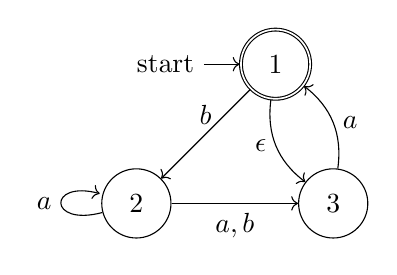
\begin{tikzpicture}[node distance = 25mm ]
    \node[state, initial, accepting] (1) {$1$};
    \node[state, below left of=1] (2) {$2$};
    \node[state, right of=2] (3) {$3$};

    \path[->] (1) edge[above] node{$b$} (2)
              (1) edge[below, bend right, left=0.3] node{$\epsilon$} (3)
              (2) edge[loop left] node{$a$} (2)
              (2) edge[below] node{$a, b$} (3)
              (3) edge[above, bend right, right=0.3] node{$a$} (1);
  \end{tikzpicture}
  \caption{An example NFA}
  \label{fig:NFA}
\end{figure}

Classically, a \emph{nondeterministic finite automaton} (NFA) is a finite state machine where
transitions are labeled with characters from a fixed alphabet $\Sigma$. These
are often represented formally as a 5-tuple $(Q, \Sigma, \delta, q_{0}, F)$,

\begin{itemize}
  \item $Q$ a finite set of states
  \item $\Sigma$ a fixed, finite alphabet
  \item $\delta : Q \times (\Sigma \cup \{ \varepsilon\}) \to \mathcal{P}(Q)$ the labeled transition function
  \item $q_{0} \in Q$ the start state
  \item $F \subset Q$ a set of accepting states
\end{itemize}

Intuitively, this can be thought of like a directed graph with nodes in $Q$ with
an edge $q \overset{c}{\to} q'$ whenever $q' \in \delta(q, c)$. Note that
transitions in an NFA may be labeled with the empty string $\varepsilon$ --- such
transitions are referred to as \emph{$\varepsilon$-transitions}. We may see an
example of an NFA in \cref{fig:NFA}.

From an NFA, we may construct a grammar of traces as follows:

First, we define a mutual fixed point grammar that describes the traces through the NFA.\ Then, we have another
grammar that tells us if we're currently in an accepting state of the automaton.
A parse of the NFA grammar is then a pair of a trace and the data that we're in
an accepting state.

Consider the NFA $N$ pictured in \cref{fig:NFA}. There are three states, $1$, $2$,
and $3$. We introduce a non-linear type $Q$ with three inhabitants $q_{1}$,
$q_{2}$, and $q_{3}$ to represent each of these states, respectively. Given a
$q, q'$, we can
then define the type of traces from $q$ to $q'$. For instance, let's construct
the traces starting at $q_{1}$ and ending at $q_{2}$ as an example.

\begin{equation}
  \label{eq:nfatrace}
  \mathsf{Trace}_{N}(q_{1}, q_{2}) = \mu
  \begin{pmatrix}
    g_{q_{1}} := g_{q_{3}} \oplus ( b \otimes g_{q_{2}} ) \\
    g_{q_{2}} := ( a \otimes g_{q_{2}} ) \oplus ( a \otimes g_{q_{3}} ) \oplus ( b \otimes g_{q_{3}} ) \oplus I \\
    g_{q_{3}} := a \otimes g_{q_{1}} \\
  \end{pmatrix}. g_{q_{1}}
\end{equation}

We should read this as defining three mutually recursive grammars, one for each
state. The definitions of these mutually recursive grammars capture the
transitions of the automaton. To ensure that we only encode traces that end in
state 2, we only include the unit $I$ as a summand in
$g_{q_{2}}$. That is, by only including $I$ at this location, it makes it the
only place where derivations of $\mathsf{Trace}(q_{1}, q_{2})$ can terminate. We
can think of all of these definitions underneath
of the $\mu$ binder as bringing some local grammars into scope. With these local
grammars in scope we are ultimately constructing a term of type $g_{q_{1}}$ to denote
only traces starting in state 1.

To encode the acceptance criteria of $N$, we want to internalize a proposition
over each state of the NFA.\ That is, for each $q \in Q$ we define a term

\[
  \mathsf{acc}(q) := q \text{ is accepting}
\]

In this example, $\mathsf{acc}(q_{1}) = \top$ and
$\mathsf{acc}(q_{2}) = \mathsf{acc}(q_{3}) = \bot$. An accepting trace of the NFA $N$ is then given by the following dependent grammar,
\[
 \mathsf{AccTrace}_{N} := \LinSigTy q Q {\left( \mathsf{Trace}_{N}(q_{0} , q) \amp \mathsf{acc}(q) \right)}
\]

where $q_{0}$ is the initial state. That is, a trace is accepted by the NFA if
we can construct the trace, and the trace ends at an accepting state. This idea
is simple enough and aligns with how we intuitively treat these automata.

Generalizing over the above example, we want to define the type of traces as,

\[
  \mathsf{Trace}_{N}(q_{0}, q_{1}) = \mu
  \begin{pmatrix}
    g_{q} := \mathsf{Trans}(q), & q \neq q_{1} \\
    g_{q} := \mathsf{Trans}(q) \oplus I , & q = q_{1}
  \end{pmatrix}. g_{q_{0}}
\]

where $\mathsf{Trans}(q)$ is an iterated disjunction that describes which
transition you should take. For an NFA, $\mathsf{Trans}(q)$ must take on the
following syntactic form,

\begin{gather*}
 \mathsf{State} \in \{ g_{q} : q \in Q \} \\
 \mathsf{Char} \in \Sigma \\
 \mathsf{Trans}_{N}(q) ::= \mathsf{Char} \otimes \mathsf{State}~|~\mathsf{State}~|~\mathsf{Trans}_{N}(q) \oplus \mathsf{Trans}_{N}(q)
\end{gather*}

That is, $\mathsf{Trans}(q)$ is a disjunction of literals followed by grammars
that encode states.

When conducting proofs involving NFA grammars, we often to
need either construct terms of type $\mathsf{Trace}_{N}(q , q')$. To
this end, we give three admissible rules for constructing
traces,

\begin{figure}[h!]
  \label{fig:admissibleintro}
  \begin{mathpar}
    \inferrule
    {~}
    {\Gamma ; \cdot \vdash \mathsf{nil} : \mathsf{Trace}_N
      (q , q)}

    \and

    \inferrule
    {\Gamma ; \Delta \vdash M : \mathsf{Trace}_N
      (dst , q') \\
    \exists \text{ transition } src \overset{c}{\to} dst
    }
    {\Gamma ; x : c , \Delta \vdash \mathsf{cons}(M) : \mathsf{Trace}_N
    (src , q')}

    \and

    \inferrule
    {\Gamma ; \Delta \vdash M : \mathsf{Trace}_N (dst , q')
      \\
    \exists~\varepsilon\text{-transition } src
    \overset{\varepsilon}{\to} dst}
    {\Gamma ; \Delta \vdash \mathsf{\varepsilon cons}(M) : \mathsf{Trace}_N
    (src , q')}
  \end{mathpar}
  \caption{Admissible Trace Constructors}
\end{figure}

That is, we may use $\mathsf{nil}$ to terminate a trace that
begins and ends at state $q$. The rules $\mathsf{cons}$ and
$\mathsf{\varepsilon cons}$ are then used to inductively
stitch traces together when sound. For instance, we can read
the $\mathsf{cons}$ rule as saying that we can
create a trace coming from a state $src$ provided that we may first
transition via the character $c$ to state $dst$ and
inductively build a trace starting from $dst$. The
$\mathsf{\varepsilon cons}$ rule says something similar, but
with an $\varepsilon$-transition instead of a transition
labelled by a character. Recall that
these rules are \emph{admissible}. They are not strictly
necessary as primitives to conduct our proofs; however, they
do provide convenient shorthand notation for building terms
of type $\mathsf{Trace}_{N}(q , q')$.

Dual to constructing traces, we often want to construct
other terms in a context containing values of type
$\mathsf{Trace}_{N}(q , q')$. For this purpose, we make use
of the elimination principle for multiple-fixed points ---
which we write as $\mathsf{mfold}$ --- given
in \cref{subsubsec:other}.

Note that this general construction will readily generalize to other types of
automata. If we wanted to define say deterministic finite automata\footnote{DFAs
\emph{could} just be defined as NFAs that happen to be deterministic. This is
one way to do so, or you may choose to present the transition relation for the
automaton as a transition \emph{function} instead. Concerns like these don't
matter so much when defining things on paper, but at formalization time these
are important and can make some proofs much easier.}, pushdown automata, Turing
machines, etc, we just swap out the type of traces for a different, but very
similar, trace construction.

With this setting for finite automata, we can now internalize some classical theorems inside of our formal system.


\subsection{A DFA Parser}
\label{subsec:regexparser}

Just as we encoded traces of NFAs as grammars, we likewise
encode the traces of a DFA as grammars. The key difference
between NFAs and DFAs is \emph{determinism} --- meaning,
that in a state $q$ inside of DFA, given a character $c$ there
will be exactly one transition that we may take leaving $q$
with label $c$. For us, this changes the definition of valid
transitions for a DFA, instead of the definition of
$\mathsf{Trans}$ provided in \cref{subsec:finiteaut} DFAs
obey

\begin{gather*}
 \mathsf{State} \in \{ g_{q} : q \in Q \} \\
 \mathsf{Trans}(q) ::= \bigoplus_{c \in \Sigma} (c \otimes \mathsf{State})
\end{gather*}

Meaning, each state has a transition for every character.

We now wish to define a parser term for DFA grammars. In
particular, for a DFA $D$ we want to build a term,

\[
  w : \String \vdash \mathsf{parse}_{D} : \mathsf{AccTrace}_{D} \oplus \top
\]

where left injection into the output type denotes acceptance
by the parser, and right injection denotes rejection. To
build such a parser, it will suffice to construct a term

\[
  w : \String \vdash \mathsf{parse}_{D} : \LinSigTy q Q {\mathsf{Trace}_{D}(q_{0} , q)}
\]
This is because given a trace of a DFA, we may easily check
if we should accept or reject by simply testing
if the final state is accepting.

Because $w$ is a Kleene star of characters, we may construct
our desired $\mathsf{parse}_{D}$ term as a $\mathsf{foldl}$
over $w$. In the empty case, we just have the trace that
ends at the accepting state. In the recursive case, we
effectively add to our trace by transitioning one character
at a time, as we read them moving across $w$.

% \todoin{Derivation tree for this construction}

Perhaps this derivation is not too surprising. All it says
is that a DFA may be ran by transitioning a single character
at a time, and then accepting or rejecting based on the
final state. This is exactly what DFAs did initially, so
what did we gain? Well, this has the benefit of our type
system to ensure its correctness. Moreover, this construction exports to an
intrinsically verified and executable DFA via Agda.


\subsection{Regular Grammars and DFAs}
\label{subsec:deriv}

In order to extend the DFA
parser from \cref{subsec:regexparser} to the construction of
a verified parser
generator for regular grammars we need to perform some
plumbing establishing an equivalence between regular
expressions and DFAs.

There are several routes we may hope to take in establishing
this equivalence. First, we could prove an equivalence
between NFAs and regular expressions, and separately prove
an equivalence between NFAs and DFAs.
In \cref{subsec:eqproofs}, we include a version of
Thompson's construction --- which established the
equivalence between regular grammars and DFAs. We may additionally
hope to internalize a variant of the powerset construction \cite{rabinFiniteAutomataTheir1959}
--- which takes as input an NFA and constructs a DFA that
recognizes the same language --- and combine the results of
Thompson's construction and the powerset constructions to give an equivalence
between regular expressions and DFAs.  This route is alluring, as it
internalizes several classic grammar-theoretic constructions. However, it may
necessitate extensions to the LNL theory, like
a propositional truncation, and we have not yet investigated
how this would interact with the existing types in the
theory. The addition of a propositional truncation may seem
harmless, but it is not always immediately clear how
distinct constructions will interact. For instance, when
exploring LNL models, Benton discovered that the synthesis
of linear and dependent types require a new presentation of
the $!$ modality from linear logic
\cite{bentonMixedLinearNonlinear1995}. That is all to say,
this is a work in progress and
it is not immediate that the addition of a propositional
truncation is adequate for establishing the weak equivalence
between NFAs and DFAs.

We may instead hope to internalize an equivalence between
regular grammars and DFAs by using Brzozowski derivatives to
directly create a DFA that is weakly equivalent to a given
regular expression, as described by Owens et al.
\cite{owensRegularexpressionDerivativesReexamined2009}.
One characterization of regular grammars is that they are
precisely those grammars which have finitely many inequivalent Brzozowski
derivatives
\cite{brzozowskiDerivativesRegularExpressions1964}.
The algorithm used by Owens takes in a
regular grammar and generates a DFA that recognizes the same
language, and the states in this DFA are the finitely many
derivative equivalence classes. We initially had a version of
this theorem very roughly internalized in the LNL theory.
To our taste, too much of this presentation relied on
meta-arguments that lived outside of
our formalism, and thus this particular phrasing of the
theorem did not translate well into formalization.

In any case, we believe
that revisiting these lines of thought will lead to a
satisfactory internalization of the equivalence between
regular grammars and DFAs, and thus would bridge the gap
between our DFA parser and a full regular expression parser.

\subsection{Equivalence Between Regular Grammars and Finite Automata}
\label{subsec:eqproofs}
In this section, we describe a version of Thompson's
construction \cite{thompsonProgrammingTechniquesRegular1968}
   where we construct an NFA that recognizes a given regular
expression. Moreover, we will show that this NFA is strongly equivalent to the
original grammar. Witnessing this construction in our syntax has two benefits
\begin{enumerate}
  \item It reinforces this high-level view that the syntax is a natural and
        general setting for formal grammar reasoning, as we demonstrate that
        this formal system subsume results from existing systems, and
  \item Following the
        development of Thompson's construction, we then need
        only establish the equivalence of NFAs and DFAs to
        complete the full regular expression parser
\end{enumerate}

\begin{theorem}[Thompson]
  \label{thm:thompson}
  For $g$ a regular grammar $g$, there is an NFA $N$ that recognizes the same
  language as $g$.
\end{theorem}
\steven{In Agda as a weak equivalence right now}

We make a pretty straightforward adaptation of Thompson's theorem to our setting,

\begin{theorem}[Typed Thompson]
  \label{thm:typthompson}
  For $g$ a regular grammar $g$, there is an NFA $N$ such that $g$ is isomorphic
  to $\mathsf{AccTrace}_{N}$.
\end{theorem}

\begin{proof}[Proof Sketch]
  The following proof is currently formalized in Agda. Below
  we give a walk through the structure of the proof.

  Recall that regular grammars are inductively defined via
  disjunction, concatenation, and Kleene star over literals
  and the empty grammar. By induction over regular grammars,
  we will construct an NFA that is equivalent to $g$.

  First, define the recognizing NFA for the empty grammar
  $I$.

  \begin{figure}[h!]
  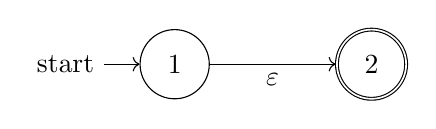
\begin{tikzpicture}[node distance = 25mm ]
    \node[state, initial] (1) {$1$};
    \node[state, right of=1, accepting] (2) {$2$};

    \path[->] (1) edge[below] node{$\varepsilon$} (2);
  \end{tikzpicture}
  \caption{$NFA(I)$}
  \label{fig:emptyNFA}
  \end{figure}

  The type of traces from the initial state of $NFA(I)$ to the single
  accepting state is given by,

  \[
    \mathsf{Trace}_{NFA(I)}(q_{1}, q_{2}) = \mu
      \begin{pmatrix}
         g_{q_{1}} := g_{q_{2}} \\
         g_{q_{2}} := I
      \end{pmatrix}. g_{q_{1}}
  \]

  The accepting traces through $NFA(I)$ are then described
  as,

  \[
    \mathsf{AccTrace}_{NFA(I)} = \LinSigTy q {\{1 , 2\}} {\left( \mathsf{Trace}_{NFA(I)}(q_{1} , q) \amp \mathsf{acc}(q) \right)}
  \]

  A quick inspection of \cref{fig:emptyNFA} reveals that the
  only reasonable choice for $q$ is $q_{2}$ --- because
  state 2 is accepting while state 1 is not. Therefore,

  \begin{align*}
    \mathsf{AccTrace}_{NFA(I)}
    & \cong \mathsf{Trace}_{NFA(I)}(q_{1} , q_{2}) \amp \mathsf{acc}(q_{2}) \\
    & \cong \mathsf{Trace}_{NFA(I)}(q_{1} , q_{2}) \amp \top \\
    & \cong \mathsf{Trace}_{NFA(I)}(q_{1} , q_{2})
  \end{align*}

  From here, to prove
  $I \cong \mathsf{AccTrace}_{NFA(I)}$ it suffices to show
  $I \cong \mathsf{Trace}_{NFA(I)}(q_{1} , q_{2})$. Below we
  give two parse transformers, one from $I$ to
  $\mathsf{Trace}_{NFA(I)}(q_{1} , q_{2})$ and vice versa. The formalized
  artifact provides the low-level details that these are
  indeed mutually inverse.

  \[
    \inferrule
    {p : I \vdash \mathsf{nil} : \mathsf{Trace}(q_{2} , q_{2}) \\
     \exists \text{~transition~} q_{1} \overset{\varepsilon}{\to} q_{2}
    }
    {p : I \vdash \mathsf{\varepsilon cons}(\mathsf{nil}) : \mathsf{Trace}_{NFA(I)}(q_{1} , q_{2})}
  \]

  Let $\gamma$ be the substitution $\{ g_{q_{2}} / g_{q_{1}}, I / g_{q_{2}} \}$,

  \[
    \inferrule
    {
      p : \mathsf{Trace}_{NFA(I)}(q_{1} , q_{2}) \vdash p :
        \mathsf{Trace}_{NFA(I)}(q_{1} , q_{2}) \\
      x_{1} : \simulsubst {g_{q_{2}}} {\gamma} = I \vdash x_{1} : I \\
      x_{2} : \simulsubst {I} {\gamma} = I \vdash x_{2} : I
    }
    {
      p : \mathsf{Trace}_{NFA(I)}(q_{1} , q_{2}) \vdash \mathsf{mfold}(x_{1}.x_{1} , x_{2}.x_{2})(p) : I
    }
  \]

  This concludes the proof for the case of the empty
  grammar. Let's now walk through the construction for
  literal grammars. Given a character $c$, we construct an
  NFA that recognizes only the string containing the single
  character $c$ as,


  \begin{figure}[h!]
  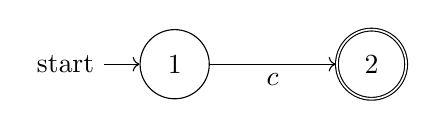
\begin{tikzpicture}[node distance = 25mm ]
    \node[state, initial] (1) {$1$};
    \node[state, right of=1, accepting] (2) {$2$};

    \path[->] (1) edge[below] node{$c$} (2);
  \end{tikzpicture}
  \caption{$NFA(c)$}
  \label{fig:literalNFA}
  \end{figure}

  The automaton in \cref{fig:literalNFA} induces the
  following type of traces from $q_{1}$ to $q_{2}$.

  \[
    \mathsf{Trace}_{NFA(c)}(q_{1}, q_{2}) = \mu
      \begin{pmatrix}
         g_{q_{1}} := c \otimes g_{q_{2}} \\
         g_{q_{2}} := I
      \end{pmatrix}. g_{q_{1}}
  \]

  Through the same argument as the empty grammar, the only
  state that is accepting is $q_{2}$ and thus,

  \[
    \mathsf{AccTrace}_{NFA(c)} \cong \mathsf{Trace}_{NFA(c)}(q_{1} , q_{2})
  \]

  To show the desired isomorphism of $c \cong NFA(c)$ we
  make a similar argument as we did for the empty grammar
  $I$, except we leverage the $\mathsf{cons}$ rule instead
  of $\mathsf{\varepsilon cons}$. That is, the parse
  transformers in either direction are given as,

  \[
    \inferrule
    {\cdot \vdash \mathsf{nil} : \mathsf{Trace}(q_{2} , q_{2}) \\
     \exists \text{~transition~} q_{1} \overset{c}{\to} q_{2}
    }
    {p : c \vdash \mathsf{cons}(\mathsf{nil}) :
      \mathsf{Trace}_{NFA(c)}(q_{1} , q_{2})}
  \]


  \[
    \inferrule
    {
      p : \mathsf{Trace}_{NFA(c)}(q_{1} , q_{2}) \vdash p :
        \mathsf{Trace}_{NFA(c)}(q_{1} , q_{2}) \\
      x_{1} : \simulsubst {(c \otimes g_{q_{2}})} {\gamma} = c \otimes I \vdash \mathsf{unitR}(x_{1}) : c \\
      x_{2} : \simulsubst {I} {\gamma} = I \vdash x_{2} : I
    }
    {
      p : \mathsf{Trace}_{NFA(c)}(q_{1} , q_{2}) \vdash \mathsf{mfold}(x_{1}.\mathsf{unitR}(x_{1}) , x_{2}.x_{2})(p) : c
    }
  \]

  Where $\gamma$ is the substitution
  $\{ c \otimes g_{q_{2}} / g_{q_{1}}, I / g_{q_{2}} \}$ and
  $\mathsf{unitR}$ is a witness to the isomorphism
  $c \otimes I \cong c$. Again, we may see that these do
  indeed mutually invert each other in the Agda code.

  It remains to show that the desired isomorphisms are
  preserved by $\otimes$, $\oplus$, and Kleene star. Here,
  we will give the argument for the disjunction case, the
  others are defined quite similarly.

  Given two NFAs $N$ and $M$, we may define a new NFA that
  encodes the disjunction of $N$ and $M$. Denote the
  internal states of $N$ by $q_{j}$'s and the internal states
  of $M$ by $r_{k}$'s,

  \begin{figure}[h!]
  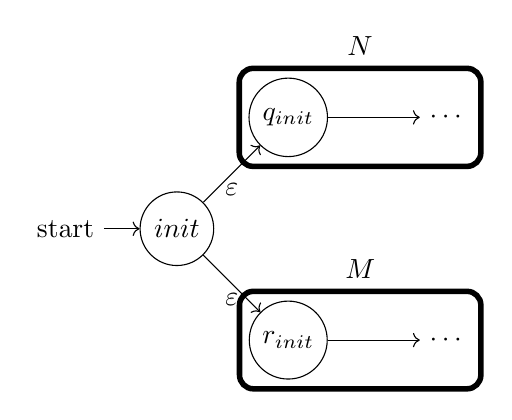
\begin{tikzpicture}[node distance = 20mm ]
    \node[state] (2) {$q_{init}$};
    \node[state, initial, below left of=2] (1) {$init$};
    \node[state, below right of=1] (3) {$r_{init}$};
    \node[right of=2] (4) {$\cdots$};
    \node[right of=3] (5) {$\cdots$};
    % \node[state, below right of=1] (3) {$3$};
    % \node[state, below of=2] (4) {$4$};

    \path[->] (1) edge[below] node{$\varepsilon$} (2);
    \path[->] (1) edge[below] node{$\varepsilon$} (3);
    \path[->] (2) edge[below] node{} (4);
    \path[->] (3) edge[below] node{} (5);

    \node[label={[name=l] $N$}, draw,line width=2pt,rounded corners=5pt, fit=(2)(4)] {};
    \node[label={[name=l] $M$}, draw,line width=2pt,rounded corners=5pt, fit=(3)(5)] {};
  \end{tikzpicture}
  \caption{$N \oplus_{NFA} M$}
  \label{fig:disjunctionNFA}
  \end{figure}

  \cref{fig:disjunctionNFA} shows the process of
  disjunctively combining NFAs. Precisely, we add a single
  new state and we included copies of the states from each of $N$
  and $M$. The new state acts as the initial state and has
  $\varepsilon$-transitions to the initial states of $N$ and
  $M$. We include all of the internal transitions from $N$
  and $M$, and the accepting states of $N \oplus_{NFA} M$
  are exactly the accepting states in each subautomaton.

  Let $g$ and $g'$ be two regular grammars such that
  $g \cong NFA(g)$ and $g' \cong NFA(g')$. As a matter of
  notation\footnote{We shall similarly abuse notation for
    $\otimes$ and Kleene. That is, for a regular grammar
    $g$, when we write $NFA(g)$ we mean the NFA inductively
    built up with the NFA-analogues to the constructors that
    built up $g$.}, we will write $NFA(g \oplus g')$ for
  $NFA(g) \oplus_{NFA} NFA(g')$. The traces of
  $NFA(g \oplus g')$ are then given by,

  \[
    \mathsf{Trace}_{NFA(g \oplus g')}(src , dst) = \mu
      \begin{pmatrix}
        g_{init} := g_{q_{0}} \oplus g_{r_{0}} \\
        g_{q_{j}} := \mathsf{Trans}_{NFA(g)}(q_{j}) \oplus \mathsf{isDst}(q_{j}) \\
        g_{r_{k}} := \mathsf{Trans}_{NFA(g')}(r_{k}) \oplus \mathsf{isDst}(r_{k})
      \end{pmatrix}.g_{src}
    \]

  where $\mathsf{Trans}$ is used to echo the same syntactic
  definitions that appear in the $NFA(g)$ and $NFA(g')$.
  Also, $src$ and $dst$ may take on any value in
  $Q := \{init\} \cup \{q_{j}\} \cup \{r_{k}\}$, and
  $\mathsf{isDst}(q)$ checks if $q$ is equal to $dst$. Which
  is all to say, the traces of $NFA(g \oplus g')$ comprise
  either a trace of $NFA(g)$, or a trace of $NFA(g')$, and
  the transition coming out of $g_{init}$ determines which
  subautomaton we step into.

  The parse transformer from $g \oplus g'$ checks which side
  of the sum type we are on, then takes the appropriate step
  from $g_{init}$ in the automaton.

  \[
    \inferrule
    {
      u : g \vdash \iota (\phi (u)) : \mathsf{AccTrace}_{NFA(g \oplus g')} \\
      v : g' \vdash \iota' (\psi (v)) : \mathsf{AccTrace}_{NFA(g \oplus g')}
    }
    {p : g \oplus g' \vdash \mathsf{case}~p \{ \mathsf{inl}(u) \mapsto s , \mathsf{inr}(v) \mapsto r \} : \mathsf{AccTrace}_{NFA(g \oplus g')}}
  \]

  with $\iota$ and $\iota'$ as embeddings from $NFA(g)$ and
  $NFA(g')$, respectively, into $NFA(g \oplus g')$,
  $\phi: g \cong \mathsf{AccTrace}_{NFA(g)}$, and $\psi: g' \cong \mathsf{AccTrace}_{NFA(g')}$. On a
  high level, all this construction does is turn a parse of
  $g$ into a parse of $NFA(g)$ and then embeds that inside
  of the larger automaton $NFA(g \oplus g')$. Likewise for $g'$.

  In the other direction, recall that the data of an
  accepting trace for $NFA(g \oplus g')$ is a pair of a
  trace and a proof that
  the end state $q'$ of that trace is accepting. By
  multifolding over the first part of that pair, we turn the
  term of type
  $\mathsf{Trace}_{NFA(g \oplus g')}(init , q')$ into a
  trace of either of the subautomata,

  \[
    p : \mathsf{Trace}_{NFA(g \oplus g')}(init , q') \vdash \mathsf{mfold}_{NFA(g \oplus g')} : \mathsf{Trace}_{NFA(g)}(q_{0} , q') \oplus \mathsf{Trace}_{NFA(g')}(r_{0} , q')
  \]

  Additionally, we leverage the fact that the only accepting
  states for $NFA(g \oplus g')$ are those from the
  subautomata to extract that $q'$ must be an accepting
  state from a subautomaton.

  \[
    x : \mathsf{acc}_{NFA(g \oplus g')}(q') \vdash M : \mathsf{acc}_{NFA(g)}(q') \oplus \mathsf{acc}_{NFA(g')}(q')
  \]

  We then combine the trace and proof of acceptance into an
  accepting trace of one of the subautomata,

  \[
    p : \mathsf{AccTrace}_{NFA(g \oplus g')} \vdash N : \mathsf{AccTrace}_{NFA(g)} \oplus \mathsf{AccTrace}_{NFA(g')}
  \]

  Lastly, we then inductively use the isomorphisms $\phi$
  and $\psi$ to turn the accepting traces into a parse of
  $g$ or $g'$,

  \[
     N : \mathsf{AccTrace}_{NFA(g)} \oplus \mathsf{AccTrace}_{NFA(g')} \vdash \mathsf{case}~N~\{\mathsf{inl}(n) \mapsto \phi^{-1}(n), \mathsf{inr}(n') \mapsto \psi^{-1}(n')\} : g \oplus g'
  \]

  As discussed above, the other cases and low-level details
  of isomorphism are reserved for the formalization. This
  concludes the proof of our variant of Thompson's construction.
\end{proof}

\subsection{Other Automata}
\subsubsection{Pushdown Automata}
\label{subsubsec:pda}
A (nondeterministic) \emph{pushdown automaton} is an automaton that employs a
stack. Just like NFAs, they have transitions labeled with characters from a
fixed string alphabet $\Sigma$. Additionally, they maintain a stack of
characters drawn from a stack alphabet $\Gamma$. They are often represented
formally as a 7-tuple $(Q, \Sigma, \Gamma, \delta, q_{0}, Z, F)$,

\begin{itemize}
  \item $Q$ a finite set of states
  \item $\Sigma$ a fixed, finite string alphabet
  \item $S$ a fixed, finite stack alphabet
  \item
        $\delta \subset Q \times (\Sigma \cup \{ \varepsilon \}) \times S \to \mathcal{P}(Q \times S^{*})$
        the transition function
  \item $q_{0} \in Q$ the start state
  \item $Z \in S$ the initial stack symbol
  \item $F \subset Q$ the accepting states
\end{itemize}

We encode the traces of a pushdown automaton very similarly to those of an NFA,
except the transitions of a PDA are instead encoded via the linear-non-linear
$\Pi$-type. This is because of simply transitioning via character, a PDA must
also pop and push characters onto a stack, which is used as the argument to
these dependent functions.

Let $S$ be a non-linear type encoding the stack
alphabet, and build lists over $S$ as the (non-linear) least fixed-point
$\mathsf{List}(S) := \mu X . 1 + S \times X$. Then, the type of states for a
PDA $P$ with stack alphabet $S$ are given as a functions that takes in lists $L$,
and then makes a case distinction between possible transitions based on what was witnessed as $\mathsf{head}(L)$. The choice of transition
will then determine which character to transition by and what word $w$ should be
pushed onto the stack. The word that is added to the top of the stack is
appended to $\mathsf{tail}(L)$ and then we recursively step into another state
called on argument $w + \mathsf{tail}(L)$.

% \begin{gather*}
%   \mathsf{State} \in {g _{q} : q \in Q} \\
%   \mathsf{Word} \in \String \\
%   \mathsf{Char} \in \Sigma   \\
%   \mathsf{StackChar} \in \Gamma \\
% \end{gather*}
% \begin{align*}
%   \mathsf{Trans}_{P}(q) ::=~&
%                            \LinPiTy {(hd :: tl)} {\mathsf{List}(S)} {\left( \mathsf{Char} \otimes \mathsf{State}(\mathsf{Word} + tl) \right)}~| \\
%   & \LinPiTy {(hd :: tl)} {\mathsf{List}(S)} {\left(  \mathsf{State}(\mathsf{Word} + tl) \right)}~|~\mathsf{Trans}_{P}(q) \oplus \mathsf{Trans}_{P}(q)
% \end{align*}

% That is to say, when transitioning a PDA pops off the head $hd$ of the stack

\subsubsection{Turing Machines}
\label{subsubsec:tm}

In
\cref{subsubsec:pda}, we gave a grammar presentation of
traces through a PDA by using a non-linear type $S$
to encode the stack. We may similarly use pairs $S \times S$
to encode the tape of a Turing machine. With two stacks we can simulate the behavior of the
infinite tape of a Turing machine. The intuition behind this correspondence is
that the left half of the tape is on one stack, the right
half of the tape the other, and we treat the tops of stacks
like the head of the tape.

Due to computability limitations, we are not able to extract
a verified parser for all recursively enumerable languages.
Yet we should still reflect on the generality of our syntax,
as it allows a natural encoding of Turing machines.

\section{Related work}
\label{sec:related}

\paragraph{Kleene Algebra}

Since the early works in the theory of formal languages, Kleene
algebras have played an important role in its development. They
generalize the operations known from regular languages by introducing
operations generalizing language composition, language union and the
Kleene star.  More generally, they are defined as inequational theory
where the inequality is meant to capture language containment. This
theory is extremely successful, having found applications in algebraic
path problems, theory of programming languages, compiler optimizations
and more.

A frequently fruitful research direction is exploring varying
extensions of Kleene algebras, Kleene algebra with tests (KAT) being
one of the most notable ones. Our approach is radically different from
most extensions, which usually aim at modifying or adding new
operations to Kleene algebras, but still keeping it as an inequational
theory. By adopting a category-theoretic treatment and allowing the
``order structure'' to encode more information than merely
inequalities, we were able to extend Kleene algebra to reason about
parsing as well.

\paragraph{TODO: more stuff}

%% That paper with Fritz Henglein about regexes as types

%% Vaughan Pratt on the residual operator
%%

\section{Future Work}
\label{sec:future}

\subsection{Implementation for Context-Free Grammars}
As suggested throughout the paper and briefly explored in
\cref{subsubsec:pda}, the first extension to the work in
this paper will be to bring analogous constructions to
context-free grammars and their accompanying pushdown automata.

\subsection{Beyond Strings}
\label{subsec:beyond}

While parsing typically refers to the generation of semantic
objects from string input, many tasks in programming can be
viewed as parsing of objects with more structure, such as
trees with binding structure or graphs. Fundamental to the
frontend of many
programming language implementations are type systems. In
particular, \emph{type checking}
--- analogous to language recognition --- and \emph{typed
  elaboration} --- analogous to parsing --- arise when
producing a semantic object subject to some analysis. Just
as our string grammars were given as functors from $\String$
to $\Set$, we envision adapting the same philosophy
to functors from $\String$ to \emph{trees} to craft a syntax
that natively captures typed elaboration. This suggests an
unusual sort of bunched type theory, where context extension
no longer resembles concatenation of strings but instead
takes on the form of tree constructors.

Thus far, our theory has proved useful for internalizing long-standing
grammar-theoretic constructions, but there has been decades of research
conducted since. A fruitful avenue for future work includes
testing if our formalism can also internalize more recently proposed grammar
mechanisms, such as the interval parsing grammars given by Zhang et al. \cite{zhangIntervalParsingGrammars2023}.

\newpage

\bibliographystyle{plain}
\bibliography{refs.bib}


\end{document}
